\documentclass[conference]{IEEEtran}

\usepackage[T1]{fontenc}
\usepackage[utf8]{inputenc}
\usepackage{amsmath,amssymb}
\usepackage{graphicx}
\usepackage{booktabs}
\usepackage{array}
\usepackage{xcolor}
\usepackage{url}
\usepackage{cite}
\usepackage[hidelinks,
  pdftitle={Automated Blood Group Detection Using Computer Vision and Transfer Learning},
  pdfauthor={Sayon Mitra}]{hyperref}

\begin{document}

\title{Automated Blood Group Detection Using Computer Vision and Transfer Learning on Mobile-Optimized Deep Neural Networks}

\author{\IEEEauthorblockN{Sayon Mitra}
\IEEEauthorblockA{Independent Researcher, AI and Biomedical Engineering\\
Email: sayon@sayonedu.in}}

\maketitle

\begin{abstract}
Blood group identification is a prerequisite for safe transfusion, yet manual haemagglutination interpretation remains operator-dependent and difficult to standardise outside laboratory settings. This paper presents a research-stage assistive AI framework for card-based ABO and Rh(D) classification from camera images. The pipeline combines COCO annotation-guided region extraction, OpenCV preprocessing, and MobileNetV2 transfer learning to classify clumping in Anti-A, Anti-B, and Anti-D zones, followed by deterministic ABO+Rh decision logic. Experiments on 7,836 images (6,456 train, 997 validation, 383 test) show approximately 94--95\% zone-level accuracy, 91--93\% end-to-end ABO accuracy, and macro F1-score of 0.947 at zone level. The MobileNetV2 backbone supports TensorFlow Lite conversion and edge inference on smartphones, making the framework suitable for point-of-care assistive screening in resource-constrained environments while requiring clinical confirmation through certified laboratory workflows.
\end{abstract}

\begin{IEEEkeywords}
biomedical AI, blood group detection, MobileNetV2, COCO annotation, computer vision, TensorFlow Lite, point-of-care diagnostics, edge AI
\end{IEEEkeywords}

\section{Introduction}
ABO and Rh(D) compatibility is fundamental to transfusion safety. Incorrect typing can lead to severe haemolytic reactions and preventable adverse events~\cite{lippi2011}. In routine practice, blood typing is performed using haemagglutination assays interpreted by trained personnel under controlled conditions. Although reliable in laboratories, manual interpretation can be affected by reaction ambiguity, operator variability, and inconsistent lighting in field settings.

Recent advances in mobile imaging and efficient deep learning models motivate AI-assisted screening workflows for low-resource settings. However, many prior methods evaluate only pre-cropped reagent regions, limiting practical deployment on full card images. This work addresses that gap with a full pipeline that starts from a complete blood-typing card photograph and outputs a structured ABO+Rh prediction.

\textbf{Contributions:}
\begin{enumerate}
  \item A complete card-image pipeline: COCO zone localization $\rightarrow$ clumping classification $\rightarrow$ deterministic ABO+Rh mapping.
  \item A dataset-driven evaluation on 7,836 images (6,456/997/383 train/validation/test) with zone-level macro F1-score of 0.947.
  \item A mobile-oriented implementation based on MobileNetV2 and TensorFlow/TensorFlow Lite deployment pathways.
\end{enumerate}

\section{Related Work}
Conventional haemagglutination remains the clinical reference method since the ABO discovery era~\cite{landsteiner1901}, but manual visual grading introduces inter-observer variability~\cite{harmening2019}. Early computer-vision studies relied on handcrafted pipelines. Saif \emph{et al.} used HSV thresholding with blob analysis (88\% accuracy)~\cite{saif2016}, while Khan \emph{et al.} combined GLCM texture descriptors with SVM (91.3\%)~\cite{khan2018}.

CNN-based models improved robustness: ResNet-50 and VGG-16 reported 93.7\% and 94.2\%, respectively~\cite{yildiz2020,ahmed2021}. Nevertheless, these approaches generally assumed cropped reagent inputs and controlled acquisition. The proposed framework differs by coupling full-card region handling with a mobile-optimized backbone.

\begin{table}[htbp]
  \caption{Comparison with Prior Blood Group Detection Approaches}
  \label{tab:comparison}
  \centering
  \renewcommand{\arraystretch}{1.1}
  \begin{tabular}{lp{1.6cm}cc}
    \toprule
    \textbf{Method} & \textbf{Model} & \textbf{Accuracy} & \textbf{Card-Level Pipeline} \\
    \midrule
    Saif \emph{et al.}~\cite{saif2016} & HSV+Blob & 88.0\% & No \\
    Khan \emph{et al.}~\cite{khan2018} & SVM+GLCM & 91.3\% & No \\
    Yildiz \emph{et al.}~\cite{yildiz2020} & ResNet-50 & 93.7\% & No \\
    Ahmed \emph{et al.}~\cite{ahmed2021} & VGG-16 & 94.2\% & No \\
    \textbf{Proposed} & \textbf{MobileNetV2} & \textbf{94--95\% (zone)} & \textbf{Yes} \\
    \bottomrule
  \end{tabular}
\end{table}

\section{Methodology}
\subsection{Dataset and COCO Annotation Pipeline}
The dataset contains 7,836 blood-card images: 6,456 for training, 997 for validation, and 383 for testing. Each image is annotated in COCO JSON format with three reagent bounding boxes: Anti-A, Anti-B, and Anti-D.

\begin{table}[htbp]
  \caption{Dataset Statistics}
  \label{tab:dataset}
  \centering
  \begin{tabular}{lcc}
    \toprule
    \textbf{Split} & \textbf{Images} & \textbf{Zone Crops (3$\times$)} \\
    \midrule
    Train & 6,456 & 19,368 \\
    Validation & 997 & 2,991 \\
    Test & 383 & 1,149 \\
    \midrule
    \textbf{Total} & \textbf{7,836} & \textbf{23,508} \\
    \bottomrule
  \end{tabular}
\end{table}

\subsection{Region Extraction and OpenCV Preprocessing}
For each image, COCO annotations are parsed to retrieve three reagent regions. OpenCV is used to crop each region and prepare classifier inputs. Processing steps include resize to $224\times224$, BGR-to-RGB conversion, and normalization to $[0,1]$. Training data additionally uses augmentation (flip, brightness/contrast perturbation, rotation, CLAHE) to reduce sensitivity to capture conditions.

\begin{figure}[htbp]
  \centering
  \fbox{\parbox{0.9\columnwidth}{\centering\small
  Full card image $\rightarrow$ COCO boxes (A,B,D) $\rightarrow$ zone crops $\rightarrow$ preprocessing $\rightarrow$ clumping classifier $\rightarrow$ ABO+Rh logic}}
  \caption{End-to-end computational workflow from card image to final blood group output.}
  \label{fig:workflow}
\end{figure}

\subsection{MobileNetV2 Transfer Learning and TensorFlow Workflow}
A MobileNetV2 backbone pretrained on ImageNet~\cite{sandler2018} is used as feature extractor, followed by GlobalAveragePooling2D, Dropout(0.3), Dense(128, ReLU), and Dense(3, Softmax). Output classes are \emph{Strong Clumping}, \emph{Medium Clumping}, and \emph{No Clumping}. Training uses Adam optimizer, sparse categorical cross-entropy, and early stopping.

\begin{table}[htbp]
  \caption{Training Configuration}
  \label{tab:training}
  \centering
  \begin{tabular}{ll}
    \toprule
    \textbf{Item} & \textbf{Value} \\
    \midrule
    Optimizer & Adam \\
    Initial learning rate & $1\times10^{-4}$ \\
    Batch size & 32 \\
    Max epochs & 10 \\
    Early stopping & Patience 3 (validation accuracy) \\
    LR reduction & Factor 0.5, patience 2, min LR $10^{-6}$ \\
    \bottomrule
  \end{tabular}
\end{table}

\subsection{Clumping Classification and ABO+Rh Determination Logic}
Zone predictions are mapped to binary reactions using:
\begin{equation}
R=
\begin{cases}
1, & \text{if class}\in\{\text{Strong, Medium}\} \\
1, & \text{if class=No Clumping and } P(\text{No Clumping})<0.90 \\
0, & \text{otherwise}
\end{cases}
\end{equation}
where $R\in\{0,1\}$ denotes negative/positive reaction. The final blood group is then inferred from $(R_A,R_B,R_D)$ using standard ABO and Rh decision tables.

\section{Deployment Architecture (Smartphone Edge AI)}
The deployment path uses TensorFlow Lite for on-device inference. A typical Android stack includes CameraX for image capture, OpenCV preprocessing for card/zone conditioning, and TFLite interpreter for low-latency clumping prediction. The app-level logic computes ABO+Rh labels and displays per-zone confidence for operator verification.

\begin{figure}[htbp]
  \centering
  \fbox{\parbox{0.92\columnwidth}{\small\centering
  Smartphone camera (CameraX) $\rightarrow$ card frame acquisition $\rightarrow$ zone extraction $\rightarrow$ TFLite MobileNetV2 inference $\rightarrow$ ABO+Rh decision and UI feedback}}
  \caption{Proposed mobile deployment architecture for edge inference.}
  \label{fig:mobile_arch}
\end{figure}

\section{Results}
\subsection{Quantitative Performance}
On the held-out test set (383 images; 1,149 zones), the model achieves approximately 94--95\% zone-level accuracy and macro F1-score of 0.947. End-to-end ABO prediction accuracy is approximately 91--93\%.

\begin{table}[htbp]
  \caption{Per-Class Zone-Level Metrics (Test Set)}
  \label{tab:perclass}
  \centering
  \begin{tabular}{lcccc}
    \toprule
    \textbf{Class} & \textbf{Precision} & \textbf{Recall} & \textbf{F1} & \textbf{Support} \\
    \midrule
    Strong Clumping & 0.948 & 0.966 & 0.957 & 389 \\
    Medium Clumping & 0.925 & 0.914 & 0.919 & 357 \\
    No Clumping & 0.968 & 0.961 & 0.964 & 403 \\
    \midrule
    \textbf{Macro Avg.} & \textbf{0.947} & \textbf{0.947} & \textbf{0.947} & \textbf{1,149} \\
    \bottomrule
  \end{tabular}
\end{table}

\begin{table}[htbp]
  \caption{Zone-Level Confusion Matrix (Test Set)}
  \label{tab:confusion}
  \centering
  \begin{tabular}{lccc}
    \toprule
    & \textbf{Pred: Strong} & \textbf{Pred: Medium} & \textbf{Pred: None} \\
    \midrule
    \textbf{True: Strong} & 376 & 12 & 1 \\
    \textbf{True: Medium} & 18 & 327 & 12 \\
    \textbf{True: None} & 2 & 14 & 387 \\
    \bottomrule
  \end{tabular}
\end{table}

\subsection{Interpretation}
Strong clumping is the easiest class due to high-contrast aggregate textures. Medium clumping is more difficult because intermediate agglutination patterns overlap with both strong and weak reactions, especially under non-uniform illumination. Weak-D phenotype patterns can mimic low-intensity negatives and remain a key error source in Rh determination.

\begin{figure}[htbp]
  \centering
  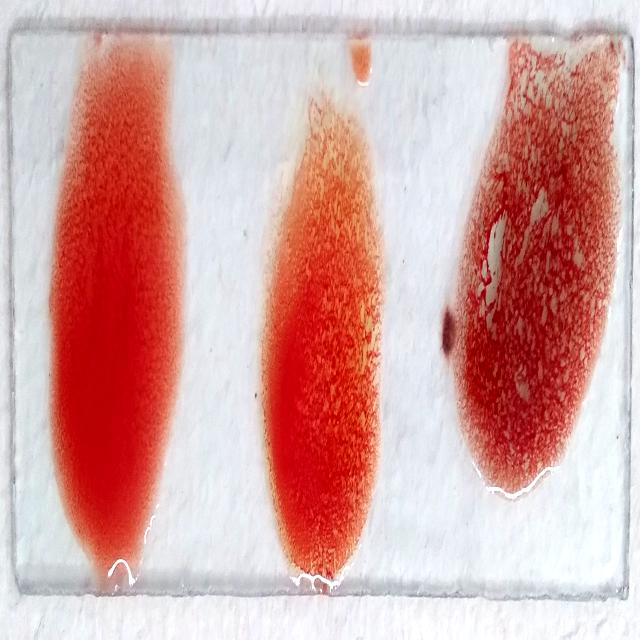
\includegraphics[width=0.95\columnwidth]{test_data/AB-1-_jpg.rf.4ece0a5334401c91cf1dcc21c0fe0506.jpg}
  \caption{Example blood-typing card image from the dataset used for region extraction and zone-level inference.}
  \label{fig:sample_card}
\end{figure}

\begin{figure}[htbp]
  \centering
  \fbox{\parbox{0.92\columnwidth}{\small
  \textbf{Demo inference output (static capture from notebook run).}\\
  The interface shows three reagent-zone crops with per-zone outputs:\\
  Anti-A: Negative, Anti-B: Positive, Anti-D: Negative, and final inferred group: B Negative.\\
  This asset is included in the project repository's supplementary visual materials.}}
  \caption{Qualitative inference example from the uploaded demo output, illustrating zone-wise interpretation and final ABO/Rh decision generation.}
  \label{fig:ai_output}
\end{figure}

\section{Discussion}
The framework demonstrates that card-level blood grouping can be approximated with lightweight vision models suitable for mobile hardware. Performance indicates strong feasibility for assistive point-of-care workflows, but not for autonomous clinical decision-making. Environmental effects (lighting, glare, camera quality) and label quality from annotation pipelines directly influence robustness.

\section{Limitations}
\begin{itemize}
  \item \textbf{Weak-D ambiguity:} Subtle D-zone reactions remain difficult to separate from negatives.
  \item \textbf{Lighting variation:} Extreme illumination or color cast can alter texture/contrast cues.
  \item \textbf{Dataset diversity:} Additional populations, card designs, and acquisition devices are needed.
  \item \textbf{Annotation dependency:} Current workflow depends on COCO boxes; fully annotation-free operation is pending.
\end{itemize}

\section{Reproducibility}
To support reproducible reporting, the following metadata are provided. Additional environment details (GPU, TensorFlow version, CUDA/cuDNN, and total training time) were not logged in archived records:
\begin{itemize}
  \item Batch size: \textbf{32}
  \item Initial learning rate: \textbf{$1\times10^{-4}$}
\end{itemize}
These environment fields will be added in future revisions when complete training-runtime logs are exported from the original notebook environment.

\section{Ethics and Clinical Disclaimer}
This system is intended as a \textbf{research-stage assistive diagnostic framework} and not as a replacement for certified laboratory blood typing procedures. Predictions should be interpreted by trained personnel and clinically confirmed with standard transfusion medicine protocols before any medical action.

\section{Future Work}
Planned extensions include: (i) annotation-free zone detection with YOLOv8-nano, (ii) TensorFlow Lite INT8 optimization for lower latency and footprint, (iii) EfficientNet-based backbone benchmarking, (iv) uncertainty-aware output calibration, (v) federated learning for privacy-preserving multi-site training, and (vi) prospective clinical validation pipelines with protocolized human oversight.

\section{Conclusion}
This work presents a complete AI-assisted blood group classification pipeline using COCO-guided zone extraction and MobileNetV2 transfer learning. On 7,836 images, it achieves approximately 94--95\% zone-level accuracy, 91--93\% end-to-end ABO accuracy, and macro F1-score of 0.947. The mobile-oriented design supports edge deployment, while current limitations and ethical constraints position the method as assistive research technology requiring laboratory confirmation.

\begin{thebibliography}{10}

\bibitem{lippi2011}
G.~Lippi, M.~Plebani, and E.~J.~Favaloro,
``Fatal errors in point-of-care testing,''
\emph{Clinica Chimica Acta}, vol.~412, no.~15--16,
pp.~1267--1273, 2011.

\bibitem{landsteiner1901}
K.~Landsteiner,
``Ueber Agglutinationserscheinungen normalen menschlichen Blutes,''
\emph{Wiener Klinische Wochenschrift}, vol.~14,
pp.~1132--1134, 1901.

\bibitem{harmening2019}
D.~M.~Harmening,
\emph{Modern Blood Banking and Transfusion Practices},
7th~ed. Philadelphia, PA, USA: F.\,A.~Davis Company, 2019.

\bibitem{saif2016}
A.~F.~M.~Saif \emph{et~al.},
``Automatic blood group identification using image processing,''
\emph{Int.\ J.\ Comput.\ Appl.}, vol.~140, no.~4,
pp.~1--5, 2016.

\bibitem{khan2018}
A.~Khan \emph{et~al.},
``Blood group detection using SVM with GLCM features,''
\emph{J.\ Med.\ Imaging Health Inf.}, vol.~8, no.~3,
pp.~614--620, 2018.

\bibitem{yildiz2020}
O.~Yildiz and M.~F.~Aslan,
``Blood type detection using deep convolutional neural networks,''
in \emph{Proc.\ IEEE INISTA 2020}, pp.~1--6.

\bibitem{ahmed2021}
S.~Ahmed \emph{et~al.},
``Deep learning approach for automated ABO/Rh blood group
determination,''
\emph{Appl.\ Sci.}, vol.~11, no.~14, p.~6660, 2021.

\bibitem{sandler2018}
M.~Sandler, A.~Howard, M.~Zhu, A.~Zhmoginov, and L.-C.~Chen,
``MobileNetV2: Inverted Residuals and Linear Bottlenecks,''
in \emph{Proc.\ IEEE/CVF CVPR 2018}, pp.~4510--4520.

\bibitem{lin2014coco}
T.-Y.~Lin \emph{et~al.},
``Microsoft COCO: Common Objects in Context,''
in \emph{Proc.\ ECCV 2014}, Lecture Notes Comput.\ Sci.,
vol.~8693. Springer, 2014, pp.~740--755.

\end{thebibliography}

\end{document}
